\section{Het verbeteren}

\subsection{Inleiding}
In de vorige deelvraag hebben we verschillende Machine Learning algoritmes behandeld. Hierbij hebben we nog niet besproken hoe een algoritme zichzelf kan verbeteren: hoe bepalen we bij Linear Regression de waarden voor $a$ en $b$ in de formule $ y = ax + b $? Hoe bepalen we de waarden voor  $x$ en $b$ in de vector $ a ∙ x - b = 0 $ bij een Support Vector Machine? Hoe bepalen we de wegingen van de synapsen in een Artificial Neural Network? Kortom: \textit{Op wat voor manieren kunnen zelflerende algoritmes zichzelf verbeteren?} Er zijn verschillende manieren waarop al deze waarden bepaald kunnen worden: Gradient Descent, Newton's method en evolutionary improvement. Deze drie leerstrategieën zullen we in deze deelvraag behandelen.

\subsection{Gradient descent}
De eerste leerstrategie die we behandelen is gradient descent. Gradient descent is een algoritme dat functies minimaliseert door het aanpassen van bepaalde parameters. Er wordt geprobeerd de waarde van een bepaalde functie zo laag mogelijk te maken. De functie die we bij een zelflerend systeem proberen te minimaliseren is de \textbf{cost function}, ook wel loss function genoemd. Dit is een functie die bepaalt hoe goed het systeem op dat moment werkt. Er wordt bepaald hoeveel de huidige outputs afwijken van de gewenste outputs. Het is hierbij dus nodig dat je de gewenste outputs weet bij gegeven inputs. Er is dus bij gradient descent altijd sprake van supervised learning. 

\subsubsection{Het algoritme} 
\begin{figure}[h]
  \centering
    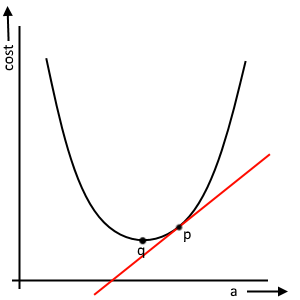
\includegraphics[width=0.5\textwidth]{GenericCostFunction.png}
  \caption{De cost function}
  \label{fig:GenericCostFunction}
\end{figure}

In figuur \ref{fig:GenericCostFunction} is de cost van een bepaalde situatie uitgezet tegen een variabele $a$. Dit kan bijvoorbeeld de $a$ uit de formule $ y = ax + b $ bij Linear Regression zijn.  Het is te zien dat de cost minimaal is in punt q. We willen dus dat a gelijk wordt aan de waarde van $a$ in punt $q$. Nu is dit punt in deze grafiek erg makkelijk te vinden, maar zodra er gebruik wordt gemaakt van een ingewikkeldere algoritme, zoals een ANN, wordt dit punt moeilijker te bepalen.


Op een gegeven moment in het trainingsproces is de $a$ gelijk aan het punt $p$. Het Gradient Descent algoritme doet dan het volgende:
\begin{itemize}
\item De afgeleide op het huidige punt wordt bepaald (de rode lijn in figuur \ref{fig:GenericCostFunction}).
\item De $a$ wordt zodanig aangepast dat het meer in de richting komt van de $q$. (Dit wordt gedaan door de afgeleide bij de variabele op te tellen)
\end{itemize}

Wanneer Gradient Descent wordt toegepast zal een bepaalde variabele in een zelflerend systeem zo aangepast worden dat de cost als gevolg van die variabele het laagst wordt. 

\subsubsection{De wiskunde achter gradient descent}
Het Machine Learning algoritme produceert met een bepaalde input een bepaalde output, dit noemen we de \textbf{guess}. Omdat we weten wat de goede ouput is kunnen we de \textbf{error} bepalen voor die input. De goede output in de volgende formule is y.

\begin{center}
$ error_{i} = y_{i} - guess_{i}$
\end{center} 

De vorige formule geldt dus voor de individuele datapunten. De totale error, de som van alle individuele error waarden, ook wel cost of loss genoemd kan als volgt beschreven worden:

\begin{center}
$ cost = \sum_{i=0}^n(error_i)^2$
\end{center}

Zoals bekend uit de wiskunde is het mogelijk om hiervan de laagste waarde te bepalen door de afgeleide op nul te herleiden. Voor elk individueel datapunt is de afgeleide van de error:

\begin{center}
$ cost_i' = 2(error_i) * error'_i$
\end{center}

Bij het differenti\"{e}ren wordt gebruik gemaakt van de kettingregel.

\subsubsection{Linear regression met gradient descent}
Om het principe van gradient descent beter te begrijpen gaan we nu door middel van gradient descent linear regression uitvoeren.

De guess is hier dus de huidige uitkomst van $ y = ax + b $.

\begin{center}
$ error_{i} = y_{i} - (xa + b)_{i}$
\end{center}

De waarde van $ b_{i} $, $ x_{i} $ en $ y_{i} $ zijn hier constant. De $ x_{i} $ en $ y_{i} $ zijn namelijk bekend uit de training data en $ b_{i} $ veranderd wel, maar niet hierbij. De afgeleide van de error functie is dan:

\begin{center}
$ error'_{i} = x_i$
\end{center}

De afgeleide van de cost function is dan:
\begin{align*}
cost_i' &= 2(error_i) * x_i \\
cost_i' &= 2(y_{i} - (xa + b)_{i}) * x_i
\end{align*}

Met de deze afgeleide is de helling van de cost function te bepalen. Hiermee dus te bepalen welke richting we de variabele a in moeten veranderen. Het aanpassen van de a bij Linear Regression gebeurt dus als volgt:

\begin{center}
$ a = a + (2 * error_i * x_i)$
\end{center}

\subsubsection{Learning rate}
Een zelflerend systeem bereikt niet in een keer de gewenste output. Er wordt langzaam in de richting van de goede output gewerkt. De formule voor het aanpassen van de $a$ waarde uit het vorige kopje is daarom iets anders. Er wordt een \textbf{learning rate} ge\"{i}ntroduceerd:

\begin{center}
$ a = a + (error_i * x_i * learning rate)$
\end{center}

Het kiezen van een goede learning rate is heel belangrijk. Een te lage learning rate zorgt ervoor dat het heel lang duurt voordat de goede output bereikt wordt. Een te hoge learning rate zorgt ervoor dat de gewenste output voorbij wordt geschoten. De gewenste output wordt dan nooit bereikt omdat de variabele net te groot of te klein wordt gemaakt. \cite{GradientDescent1}\cite{GradientDescent2}

\subsection{Newton's method}
Net zoals gradient decent is Newton's method, vernoemd naar Isaac Newton, een manier om de laagste waarde van een bepaalde functie te bepalen. Hiervoor maakt gradient descent gebruik van het gegeven dat een extreme waarde van een grafiek een richtingsco\"effici\"ent van nul heeft en de afgeleide op dat punt dus gelijk is aan nul. Newton's method gebruik voor het bepalen van de laagste waarde de tweede afgeleide. Er wordt dan gekeken op welke punten deze lijn de x-as snijdt, dit zijn namelijk de toppen van de grafiek van de eerste afgeleide. Door gebruik te maken van Newton's method, zul je een schatting krijgen van het snijpunt met de x-as, maar waarschijnlijk zal je dit punt niet exact kunnen vinden. De nauwkeurigheid van de schatting hangt af van de hoeveelheid waarmee je de stappen herhaalt.

\subsubsection{Het proces}
In figuur \ref{fig:NM1} is een willekeurige grafiek getekend.

\begin{figure}[H]
  \centering
    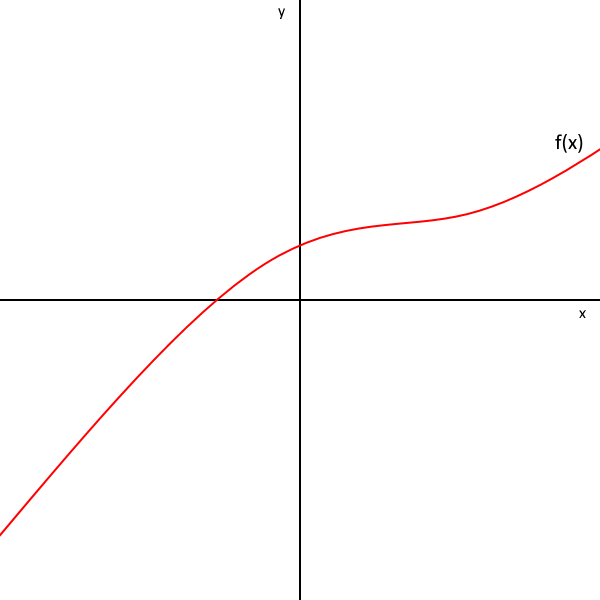
\includegraphics[width=0.5\textwidth]{NewtonsMethod1.png}
  \caption{De grafiek van een willekeurige functie $ f(x) $}
  \label{fig:NM1}
\end{figure}

Bij het gebruik van Newton’s method, waarbij we dus zoeken naar een snijpunt met de x-as, wordt eerst een gok gedaan. Deze gok, op punt $a$, correspondeert met een waarde op de grafiek van $ f(x) $. Aan dit punt wordt een raaklijn getekend.

\begin{figure}[h]
  \centering
    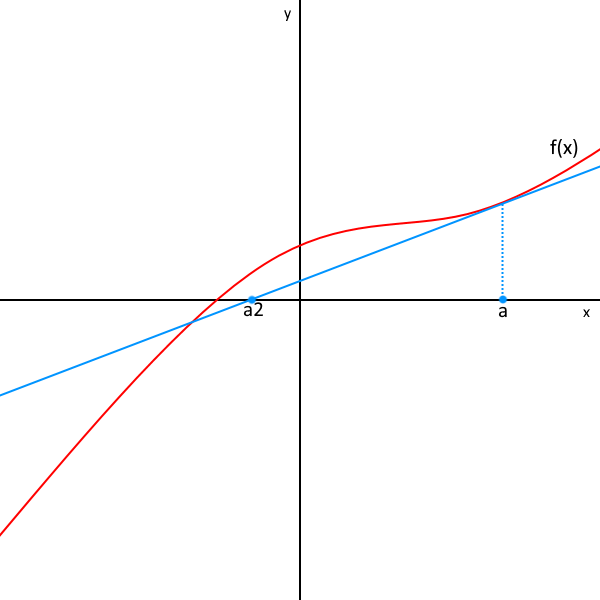
\includegraphics[width=0.5\textwidth]{NewtonsMethod2.png}
  \caption{Een raaklijn aan $ f(x) $ op punt $ x = a $}
  \label{fig:NM2}
\end{figure}

De raaklijn van $ f(x) $ op $ f(a) $ snijdt de x-as op een bepaald punt $ a_2 $. Te zien is dat dit punt al aanzienlijk dichter bij het doel ligt dan de originele schatting. Ook $ a_2 $ correspondeert met een waarde van $ f(x) $ en ook op dit punt kan weer een raaklijn getekend worden (figuur \ref{fig:NM3}).

\begin{figure}[h]
  \centering
    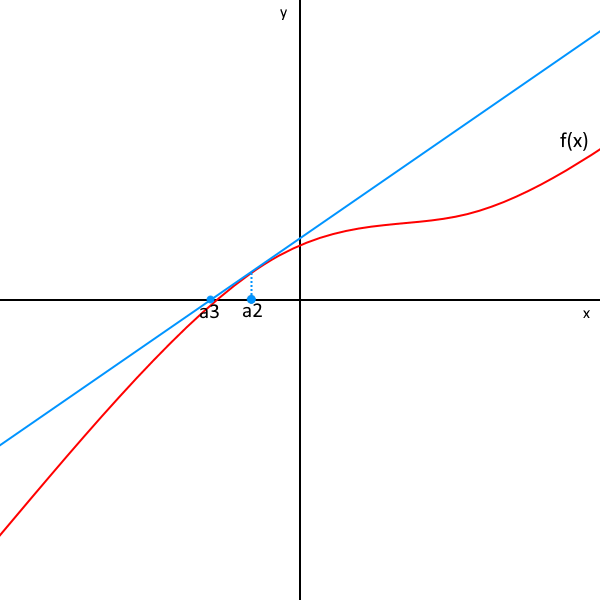
\includegraphics[width=0.5\textwidth]{NewtonsMethod3.png}
  \caption{Een raaklijn aan $ f(x) $ op punt $ x = a_2 $}
  \label{fig:NM3}
\end{figure}

Na slechts twee raaklijnen getekend te hebben, ligt het punt $ a_3 $ al erg dicht bij het doel. Om een nauwkeurigere benadering van dit doel te bereiken kan je vaker een raaklijn tekenen en het nieuwe snijpunt bepalen. Hoe nauwkeurig je een benadering wil hebben verschilt per situatie.

\subsubsection{De wiskunde}
Uiteraard zijn de waardes van de punten $ a_2 $, $ a_3 $ ... $ a_n $ te berekenen, we willen immers de waarde van het nulpunt bepalen. Dit gebeurt als volgt:

We weten dat de afgeleide de helling van de grafiek aangeeft: $ \frac{\Delta y}{\Delta x} $. Het idee is dat je de helling berekent tussen twee punten die oneindig dicht bij elkaar liggen, hier aangegeven met d: $ \frac{dy}{dx} $. Voor het gemak noemen we deze punten x en c. Dit geeft voor de afgeleide:

\begin{center}
$ f'(c) = \frac{f(x) - f(c)}{x - c}$
\end{center}

Dit kan omgeschreven worden tot de formule voor een raaklijn:

\begin{align*}
	   f'(c)(x - c) &= f(x) - f(c) \\
f'(c)(x - c) + f(c) &= f(x)
\end{align*}

Om het nulpunt te berekenen, moet gelden $ f(x) = 0 $. Omdat c slechts een andere waarde voor x aanduidde, kunnen we deze vervangen door het volgende: $ c = x_n $ en $ x = x_{n+1} $

\begin{align*}
			 f'(x_n)(x_{n+1} - x_n) + f(x_n) &= 0 \\
	f'(x_n)* x_{n+1} - f'(x_n) * x_n + f(x_n)&= 0 \\
							f'(x_n)* x_{n+1} &= f'(x_n) * x_n - f(x_n) \\
		   \frac{f'(x_n) * x_{n+1}}{f'(x_n)} &= \frac{f'(x_n) * x _n - f(x_n)}{f'(x_n)} \\
									  x_{n+1}&= x_n - \frac{f(x_n)}{f'(x_n)}
\end{align*}

Met deze formule kan de volgende waarde voor x berekend worden.

\subsubsection{Het gebruik}
Er zijn vele situaties te bedenken waarin je de nulpunten van een functie zou willen weten. In het gebied van machine learning wordt het gebruikt om te berekenen waar de cost functie minimaal is. Onder het kopje gradient descent staat al beschreven hoe we aan de cost functie komen en wat de afgeleide hier van is. De grafiek die afgebeeld staat zou de afgeleide van deze cost functie zijn. Dit betekent namelijk dat de tweede afgeleide van de cost functie wordt genomen wanneer je een raaklijn aan de grafiek berekent.

Gradient descent kan goed worden gebruikt bij grafiek met slechts \'e\'en minimum. Zodra dit niet het geval is, kan het makkelijk in een dal vast blijven hangen, denkend dat het de minimale waarde gevonden heeft, terwijl er misschien nog een lager punt te vinden is. Bij zulke gevallen kan Newton's method ingezet worden, want al deze punten zullen wel op de x-as liggen en dus zullen ze allemaal te vinden zijn met Newton's method.

\subsubsection{Newton's method uitgebeeld}
Om te Newton's method beter te begijpen en om op een andere manier met de stof bezig te zijn, hebben een programma geschreven in java dat de manier waarop Newton's method werkt, uitbeeldt. Zodra je dit programma opstart, krijg je een scherm te zien waarin je de functie die je wil onderzoeken kan invullen. Dit is te zien in figuur \ref{fig:PraktijkNewtonsMethod1}. Als je vervolgens op \textit{Start} drukt, krijg je de door jouw ingevoerde formule te zien in een assenstelsel. Druk nu op \textit{Run} om Newton's method uit te voeren. (Zie figuur \ref{fig:PraktijkNewtonsMethod2}) In de vakjes \textit{Current} en \textit{Best} staan de huidige schatting en de beste schatting van het nulpunt van de lijn weergegeven. Ten slotte heb je een knop om de ingevoerde functie te veranderen.

\begin{figure}[h]
  \centering
    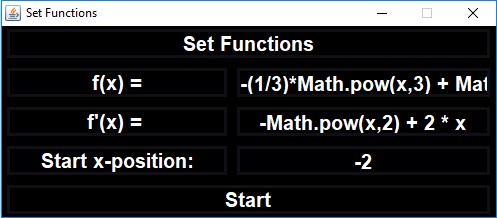
\includegraphics[width=0.5\textwidth]{PraktijkNewtonsMethod1.png}
  \caption{Het invullen van een formule in ons programma}
  \label{fig:PraktijkNewtonsMethod1}
\end{figure}

\begin{figure}[H]
  \centering
    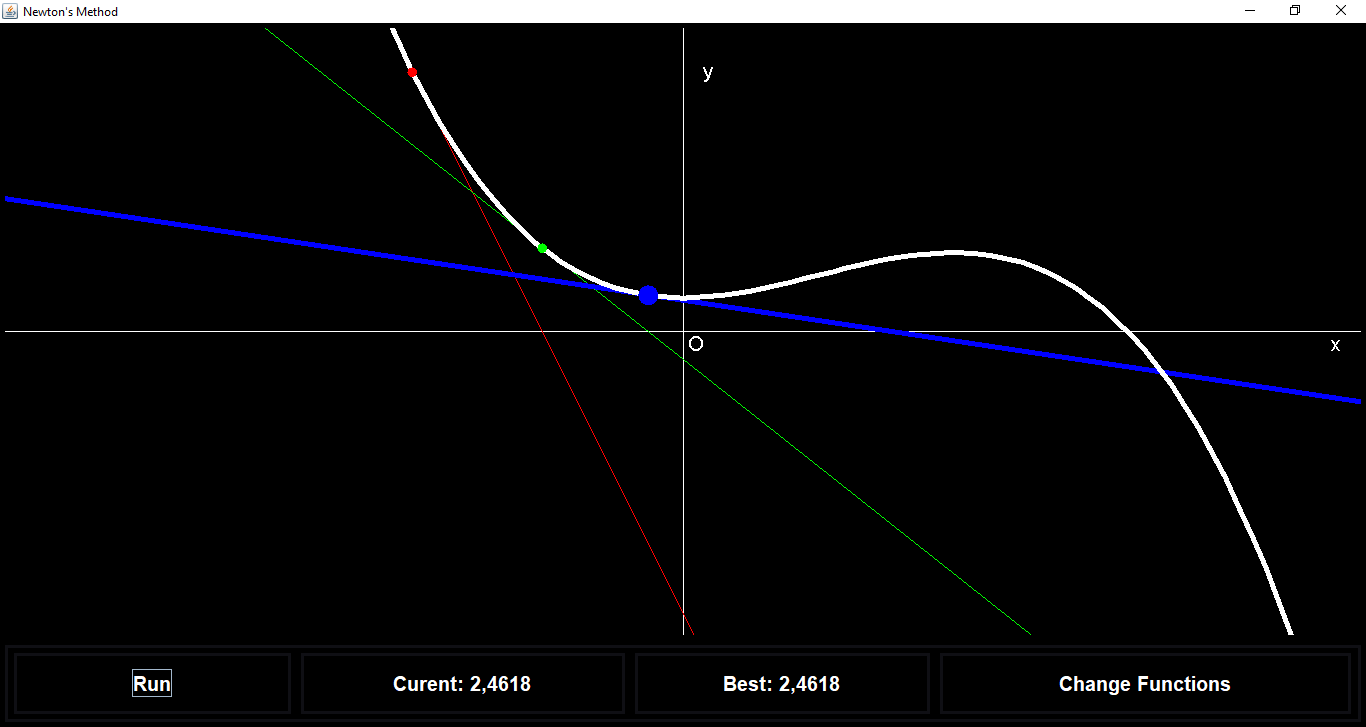
\includegraphics[width=0.7\textwidth]{PraktijkNewtonsMethod2.png}
  \caption{Newton's method uitgebeeld}
  \label{fig:PraktijkNewtonsMethod2}
\end{figure}

\subsection{Evolutionary improvement}
Het leerproces van een systeem zou de evolutie van het systeem genoemd kunnen worden: het leert zichzelf beter te functioneren in een bepaalde omgeving. Net zoals evolutie in de biologie, gaat evolutionary improvement in generaties van systemen. Deze manier van leren maakt gebruik van het doorgeven van informatie tussen deze generaties om het algemene niveau van presteren te verhogen.

\subsubsection{DNA}
Wanneer evolutionary improvement wordt toegepast, is er altijd sprake van een bepaald DNA. In dit DNA staan een aantal waardes. Deze waardes kunnen worden doorgegeven aan de volgende generatie.

\subsubsection{Een populatie}
Wanneer de informatie van een enkel individu telkens wordt doorgegeven aan een volgende generatie die ook bestaat uit slecht \'{e}\'{e}n individu, zal de verbetering van een systeem niet zo groot of zelfs afwezig zijn. Het systeem weet niet of het DNA dat doorgegeven wordt goed of slecht presteert, want er is maar \'{e}\'{e}n individu per generatie. Om deze reden bestaat een generatie meestal uit meerdere individuen. Ze zullen niet allemaal even goed presteren en dus zal er onderscheid gemaakt kunnen worden tussen goed en slecht.

De overgave van DNA kan op veel verschillende manieren gebeuren en is afhankelijk van het soort programma en de voorkeur van de programmeur. Je zou bijvoorbeeld de individuen uit een populatie kunnen rangschikken op volgorde van prestatie (hoe prestatie wordt gemeten is natuurlijk ook geheel afhankelijk van het soort programma) en een bepaald percentage van het slechtst presterende deel laten afvallen \cite{carrykh}. Vervolgens vul je dit deel weer op met individuen met een willekeurig DNA, de rest van de populatie blijft gelijk. Het idee is dat je door telkens het slechte DNA weg te filteren, uiteindelijk een populatie krijgt die gemiddeld steeds beter presteert.

Een andere manier voor evolutie is stellen dat na een bepaalde tijd elk individu een 'kind' krijgt. Dit zou goed kunnen werken in een simulatie waarin individuen een rivaliserend verband met elkaar hebben, bijvoorbeeld doordat ze dezelfde voeding nodig hebben. De individuen die langer overleven zullen meer kinderen krijgen en hun DNA dus vaker doorgeven, terwijl de individuen met slechte eigenschappen snel doodgaan. Natuurlijk kan je er ook voor kiezen het DNA van meerdere individuen te combineren voor een volgende generatie.

\subsubsection{Mutaties}
In de biologie kan in het DNA een mutatie plaatsvinden. Een mutatie is een willekeurige verandering zonder echte reden. Nu kunnen deze mutaties nadelig zijn door bijvoorbeeld ziektes te veroorzaken, maar voor evolutie zijn ze erg nuttig. Zonder mutaties zou het DNA altijd gebonden blijven aan wat er al bestaat omdat het telkens wordt doorgegeven. Zo zou er niets nieuws kunnen ontstaan en zou het systeem misschien vast komen te zitten. Als je bijvoorbeeld een programma hebt waarin een systeem leert een hindernisbaan over te gaan, maar geen enkel individu heeft in zijn DNA staan hoe je moet springen, dan kan het programma nooit over een horde heen komen. Mutaties dienen ervoor zulke problemen te voorkomen. Je voegt een bepaalde mutatiefactor toe, een kleine kans die ervoor zorgt dat het programma soms een willekeurige verandering aanbrengt waardoor nieuwe mogelijkheden voor de individuen kunnen ontstaan.

\subsection{Conclusie}
Zelflerende algoritmes kunnen zichzelf verbeteren door gebruik te maken van leerstrategien. Drie veel gebruikte leerstrategien zijn: \textit{Gradient descent}, \textit{Newton's method} en \textit{Evolutionary improvement}. De eerste twee gebruiken een wiskundige aanpak  terwijl Evolutionary improvement vooral op kans gebaseerd is.

\textcolor{praktijk}{
\subsection{Praktijk: Newton's Method}
}